\documentclass[11pt]{article}
\usepackage[T1]{fontenc}
\usepackage{lmodern}
\usepackage{microtype}
\usepackage[utf8]{inputenc}
\usepackage{amsmath,amssymb,amsthm,mathtools}
\usepackage[margin=1.1in]{geometry}
\usepackage{graphicx,booktabs,longtable,array}
\usepackage[numbers,sort&compress]{natbib}
\usepackage[colorlinks]{hyperref}
\hypersetup{pdftitle={Succinct Rabung certificates and recurrence-closed lower bounds for van der Waerden numbers},
  pdfauthor={Brice Pouly},
  pdfsubject={van der Waerden numbers},
  pdfkeywords={van der Waerden numbers, lower bounds, power residues, Rabung, GPU, certificates}}
\newtheorem{theorem}{Theorem}
\newtheorem{proposition}[theorem]{Proposition}
\newtheorem{lemma}[theorem]{Lemma}\newtheorem{conjecture}[theorem]{Conjecture}
\theoremstyle{definition}\newtheorem{definition}[theorem]{Definition}\newtheorem{remark}[theorem]{Remark}
\newcolumntype{P}[1]{>{\raggedright\arraybackslash}p{#1}}
\title{Succinct Rabung certificates and recurrence-closed\\
lower bounds for van der Waerden numbers}
\author{Brice Pouly}
\date{}
\begin{document}\maketitle
\begin{center}
\fbox{\begin{minipage}{0.90\linewidth}\small
\textbf{Qualification status (28 August 2026).}
This is a private prepublication draft, not the citable release.  Open gates
include the final 13 claim manifests, 515-chunk campaign recovery,
ordered-prime audit, CUDA qualification, four external certificate rechecks, outbound
licences, and DOI/tag freeze, as recorded in \texttt{STATUS.json}.  Numerical
statements below report the current computation; release-level reproducibility
claims remain conditional on the full ledger.
\end{minipage}}
\end{center}
\begin{abstract}
A historical single-GPU campaign was configured to scan every prime in
$[9.7\times10^{8},\,2\times10^{9})$ for power-residue colourings.  Its retained
summaries identify nine candidate direct Rabung certificates for $W(3,k)$,
$17\le k\le25$, headed by $W(3,17)>31\,385\,622\,833$.  The GPU discovers the
triples; it is not the source of the proof.  For each triple $(p,r,k)$, a
stand-alone, separate-source CPU verifier can re-establish the finite
hypotheses of Rabung's theorem from scratch.  Conditional on acceptance of the
registered claim manifests, closing a dated corpus
of published, archived, and current baselines under the recurrences of
Blankenship--Cummings--Taranchuk and Xu leaves the direct values as the
strongest bounds located there for $17\le k\le21$.  The rows
$22\le k\le25$ improve the direct Rabung family but are not general van der
Waerden records.  Retained historical runs also report separate-source
acceptance of four archived two-colour certificates due to Monroe; final
release rechecks remain open.  Applying the Blankenship--Cummings--Taranchuk
recurrence gives, in particular,
$W(3,25)>628\,673\,328\,287$ and
$W(3,28)>2\,159\,051\,058\,266$.  A secondary holdout analysis compares three
frozen forecasts with one cumulative trajectory; its disjoint increments are
primary and every Poisson calculation is conditional on the stated model.
\end{abstract}
% ============ STRUCTURE ============
\section{Introduction}\label{s:intro}

A lower bound for a van der Waerden number is witnessed by a colouring that
avoids long monochromatic arithmetic progressions. At the sizes considered
here, such a colouring contains tens of billions of positions. Its description,
however, need not be comparably large. In Rabung's power-residue construction,
a triple of integers $(p,r,k)$ determines the finite conditions from which the
colouring and its lower bound follow. The computational problem is to find a
useful triple; the mathematical problem is to verify those conditions and to
place the bound among the consequences of earlier constructions.

For integers $r\ge2$ and $k\ge3$, let $W(r,k)$ be the least $N$ such that
every $r$-colouring of $\{1,\dots,N\}$ contains a monochromatic arithmetic
progression of length $k$. We put colours first. Monroe~\cite{Monroe2026}
uses the reverse convention $W(k,r)$; Fox and Hunter~\cite{FoxHunter2026}
write $w(k;r)$.

\subsection{Numerical results and their scope}

We obtain three primitive three-colour Rabung certificates, at lengths
$17$, $18$ and $19$. They give nine direct inequalities for $17\le k\le25$;
the final six follow from the length-19 certificate by a fixed-prime
monotonicity lemma. In particular,
\[
 W(3,17)>31\,385\,622\,833,
\]
using $p=1\,961\,601\,427$. This is a factor $2.02$ above the earlier
$15\,509\,557\,937$ listed by Monroe. The five inequalities for
$17\le k\le21$ improve the prior comparators identified in the source review
updated on 26~September~2026; Table~\ref{tab:priority} gives their values.

A new direct certificate need not give a better general bound. For
$22\le k\le25$, our certificates improve the Rabung rows located in the
review, but stronger bounds already follow from other constructions. A
stronger published statement of Landman and Robertson has an unresolved
proof status in our audit. We display its consequences separately and include
it among prior comparators: the five improvements at lengths $17$--$21$
remain, whereas it dominates the admitted table at lengths $24$--$28$.
This is a comparison with a dated, explicit corpus, not an assertion of
exhaustive global priority.

We also recheck four two-colour certificates from the archived second phase of
Monroe's distributed project~\cite{MonroePhase2Archive}, retaining the credit
of that project and its volunteers. Together with the nine three-colour rows,
they form the thirteen inequalities of Theorem~\ref{thm:certified-rabung}.
Only seven triples are primitive; the archived rechecks deliberately retain
the redundant consequences.

\subsection{From a short certificate to a finite comparison}

Multiplication by a nonzero residue permutes the colour classes of a
power-residue colouring. After such a dilation, an arithmetic progression
becomes a consecutive string. Rabung's theorem reduces the large-colouring
problem to a run-length test and a condition at the multiples of
$p$~\cite{rabung1979}. A qualifying prime gives $W(r,k)>(k-1)p+1$.
We prove the equivalence of the implemented boundary test with the published
criterion and provide a stand-alone CPU checker whose source and arithmetic
are separate from the GPU search. The small example in
Section~\ref{ss:criterion} illustrates the reduction before the proof.

\begin{figure}[htbp]
\centering
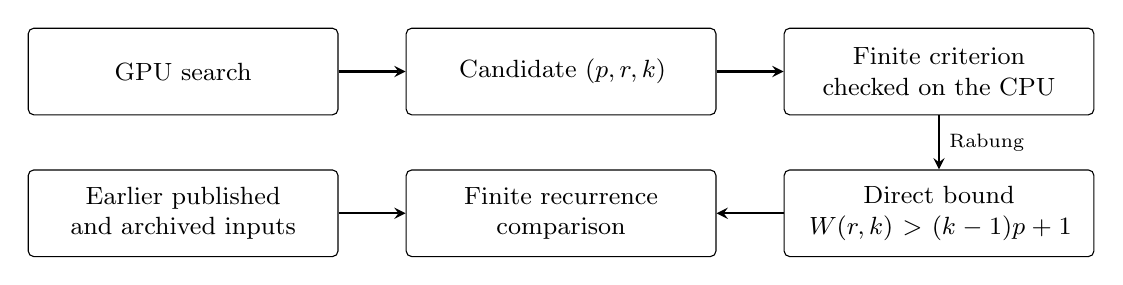
\begin{tikzpicture}[>=stealth,box/.style={draw,rounded corners=2pt,
  align=center,font=\small,minimum height=11mm,text width=3.7cm},
  edge/.style={->,thick}]
\node[box] (search) at (0,0) {GPU search};
\node[box] (triple) at (4.8,0) {Candidate $(p,r,k)$};
\node[box] (check) at (9.6,0) {Finite criterion\\checked on the CPU};
\node[box] (prior) at (0,-1.8) {Earlier published\\and archived inputs};
\node[box] (closure) at (4.8,-1.8) {Finite recurrence\\comparison};
\node[box] (bound) at (9.6,-1.8) {Direct bound\\$W(r,k)>(k-1)p+1$};
\draw[edge] (search)--(triple);
\draw[edge] (triple)--(check);
\draw[edge] (check)--node[right,font=\scriptsize]{Rabung}(bound);
\draw[edge] (bound)--(closure);
\draw[edge] (prior)--(closure);
\end{tikzpicture}
\caption{The two steps after discovery. The candidate can be checked without
replaying the search, and its bound is compared with consequences of earlier
inputs. Campaign coverage and the empirical intensity analysis are separate
from these pointwise implications.}
\label{fig:evidence-flow}
\end{figure}


Earlier bounds must then be compared under known recurrences. For example,
Blankenship, Cummings and Taranchuk~\cite[Theorem~2.1]{bct2018} prove
\begin{equation}\label{eq:bct-intro}
 W(r,k)>q\left(W\!\left(r-\left\lceil r/q\right\rceil,k\right)-1\right)
\end{equation}
for a prime $q\le k$. For three colours, an earlier strict bound
$W(2,k)>B$ gives $W(3,k)>q_kB$, where $q_k$ is the largest prime at most
$k$. This explains why a larger Rabung prime need not yield the strongest
general bound. Our finite comparison also includes length monotonicity and
the registered Xu operation~\cite{xu2013,Monroe2026}, with exact integers
and a provenance path for every retained value. No winning three-colour row
depends on Xu.

\subsection{Relation to earlier work}

Computational power-residue constructions and cyclic-zipper extensions have
been developed by Herwig, Heule, van Lambalgen and van Maaren~\cite{herwig2007},
Rabung and Lotts~\cite{rabunglotts2012}, Liang, Xu, Shao and
Xiu~\cite{liang2012}, and Monroe~\cite{Monroe2016v1,Monroe2017v4,Monroe2026}.
Publishing a prime together with checking code has antecedents in this
literature. Our contribution is the three new primitive certificates, their
separate verification, and their explicit comparison with consequences of
the identified prior inputs. Certification is not presented as a new principle.

Berlekamp's construction supplies a stronger admitted bound at length $24$,
inherited at length $25$~\cite{Berlekamp1968}. The stronger
Landman--Robertson statement requires the separate treatment just
described~\cite{LandmanRobertson2004,LandmanRobertson2014,Johannson2007}.
The recent superexponential three-colour result of Fox and
Hunter~\cite{FoxHunter2026} and the asymptotic two-colour bound
$w(k)\ge(1-o(1))k2^{k-1}$ of Campos, Fox and
Schildkraut~\cite{CamposFoxSchildkraut2026} address different asymptotic
questions. In the version-pinned sources examined, neither supplies a
stronger explicit finite entry for our window.
Gasarch and Haeupler's explicit family
$W(3,k)\ge3^{k-1}/(ek)$~\cite[Note~1.7(2)]{GasarchHaeupler2011} is retained
in the registry and is dominated there. Kozik and
Shabanov~\cite[Theorem~2 of the arXiv version]{KozikShabanov2014} give
$W(r,k)\ge\beta r^{k-1}$ for an absolute $\beta>0$; no finite improvement
from that theorem is asserted here. Hunter's exponential improvement begins
at five colours~\cite{Hunter2025} and does not change the three-colour table.

\subsection{Reading guide and evidence boundary}

Section~\ref{s:bounds} gives the numerical results and their comparison.
Section~\ref{s:method} explains the construction, proves the boundary-test
equivalence and describes the checker. Section~\ref{s:campaign} explains
the discovery and verification protocol. The search covered
$[9.7\times10^8,2\times10^9)$ in $515$ chunks; its coverage evidence has a
separate role from the validity of any one certificate.

A reader interested in the inequalities can read the results and the
criterion proof first. The witness is short, but a complete recheck still
visits a linear number of residues and evaluates their colours; checking the
identities of the retained archive is a separate, much lighter operation. The source catalogue, campaign audit and execution
identities remain available in the appendices and accompanying package.
Appendices~\ref{s:prereg}--\ref{s:densitydiagnostics} compare three fixed
search-intensity forecasts on one run-valid $(3,17)$ trajectory. That empirical
comparison neither proves a density law nor enters the lower-bound proof.
No independently administered external replication has been performed; the
preserved local computations and their limits are stated throughout.

\section{Certified direct claims and closed lower bounds}\label{s:bounds}

\subsection{Verification protocol}\label{ss:protocol}

The computational source of truth contains exactly thirteen direct Rabung
claims: nine three-colour claims for $17\le k\le25$ and four two-colour
claims for $25\le k\le28$.  For each triple $(p,r,k)$ the release protocol
requires:
\begin{enumerate}
\item two executions of the structured triplet \{mirror scan, full scan,
  CPU walk\}, with internal profile equality and equality between executions;
\item two acceptances by the separate full CPU criterion;
\item acceptance by the stand-alone \texttt{verify\_claim}; and
\item for the two primes above the historical Montgomery-safety threshold, an
  additional full-interval witness that uses no Montgomery arithmetic.
\end{enumerate}
The parser is fail-closed: it checks the process status, the exact $p,r,k$,
all profile equalities, (a), (B$^*$), and the final verdict, and rejects any
output containing \texttt{DIFF}, \texttt{FAIL}, \texttt{ECHEC}, or a negative
verdict.  Its digest engages the claim identity, profiles, criterion values,
and final verdict.  The enclosing JSON manifest separately records the source
and binary hashes, compiler version, exact commands, and hashes of every raw
output.  A SHA-256 of that manifest therefore binds the computational claim to
its build and evidence.  The final Markdown and \LaTeX{} claim tables are
generated only from an exact set of thirteen accepted manifests.

\IfFileExists{generated_validated_claims.tex}{%
  \input{generated_validated_claims}%
}{%
  \begin{center}
  \fbox{\begin{minipage}{0.91\linewidth}\small
  \textbf{Validated-claim table unavailable in this build.}
  The canonical table appears only when the exact set of thirteen fail-closed
  claim manifests is available and validated.  The publication contract
  requires the generated table in a release build.
  \end{minipage}}
  \end{center}
}

This rule is stricter than the historical campaign transcript.  The latter
recorded a max-run checksum that did not engage $p$, and some pasted
\texttt{verify\_claim} outputs were truncated.  Those files are retained as
historical evidence, not used as the final source of truth.  The thirteen
claims are documented in \texttt{audit/claims.json}; the expensive final
point-verification run must populate the complete raw manifests before the
release is frozen.  The numerical bounds in this section use only the
thirteen triples, each of which is also re-derived by the separate-source
checker described in Section~\ref{ss:certificates}.

\subsection{Three colours: direct and recurrence-derived bounds}\label{ss:r3}

The historical scan produced nine candidate direct Rabung certificates.  The headline value
\[
  W(3,17)>31\,385\,622\,833
\]
comes from $p=1\,961\,601\,427$ and improves Monroe's published
$15\,509\,557\,937$ by a factor $2.02$~\cite{Monroe2026}.  A direct certificate
is not automatically a general record: published bounds in other colour
columns may imply a stronger result through a recurrence.

Let $q_k$ denote the largest prime not exceeding $k$.  From
Blankenship--Cummings--Taranchuk~\cite[Theorem~2.1]{bct2018},
\[
  W(3,k)>q_k\bigl(W(2,k)-1\bigr).
\]
If the registered input is the strict integer bound $W(2,k)>B$, then
$W(2,k)-1\ge B$, so the generated consequence is exactly
\begin{equation}\label{eq:bct-r3}
  W(3,k)>q_k B,
\end{equation}
with no off-by-one ambiguity.  The baseline program iterates this rule and
Xu's recurrence to a fixed point, retains a provenance path for every generated
candidate, and selects the best bound only afterwards.  Its output also embeds
the source catalogue and SHA-256 hashes of both input registries.

% Generated by tools/close_baselines.py; do not edit by hand.
\begin{table}[ht]
\centering\footnotesize
\begin{tabular}{c r r r l}
\toprule
$k$ & direct $p$ & direct bound & best closed bound & method \\
\midrule
17 & $1\,961\,601\,427$ & $31\,385\,622\,833$ & $31\,385\,622\,833$ & direct Rabung \\
18 & $1\,999\,994\,851$ & $33\,999\,912\,468$ & $33\,999\,912\,468$ & direct Rabung \\
19 & $1\,999\,999\,927$ & $35\,999\,998\,687$ & $35\,999\,998\,687$ & direct Rabung \\
20 & $1\,999\,999\,927$ & $37\,999\,998\,614$ & $37\,999\,998\,614$ & direct Rabung \\
21 & $1\,999\,999\,927$ & $39\,999\,998\,541$ & $39\,999\,998\,541$ & direct Rabung \\
22 & $1\,999\,999\,927$ & $41\,999\,998\,468$ & $49\,058\,715\,046$ & BCT, $q=19$ (published $W(2,k)$) \\
23 & $1\,999\,999\,927$ & $43\,999\,998\,395$ & $142\,741\,265\,701$ & BCT, $q=23$ (published $W(2,k)$) \\
24 & $1\,999\,999\,927$ & $45\,999\,998\,322$ & $252\,542\,143\,876$ & BCT, $q=23$ (published $W(2,k)$) \\
25 & $1\,999\,999\,927$ & $47\,999\,998\,249$ & $628\,673\,328\,287$ & BCT, $q=23$ (archived input) \\
26 & -- & -- & $1\,221\,912\,599\,848$ & BCT, $q=23$ (archived input) \\
27 & -- & -- & $2\,068\,976\,009\,617$ & BCT, $q=23$ (archived input) \\
28 & -- & -- & $2\,159\,051\,058\,266$ & BCT, $q=23$ (archived input) \\
\bottomrule
\end{tabular}
\caption{Direct three-colour Rabung certificates and the best general lower bounds
obtained after closing the registered baselines under the published
Blankenship--Cummings--Taranchuk and Xu recurrences.  A dash means that the
GPU campaign made no direct three-colour claim for that length.  For
$k=22,23,24,25$ the direct certificates are the strongest direct Rabung bounds
located in the dated corpus but are not general records. Every entry is generated with a
machine-readable provenance path in \texttt{audit/generated/bounds\_closure.json}.}
\label{tab:r3}
\end{table}


Thus the direct certificates for $17\le k\le21$ remain the strongest bounds
located in the registered published-and-archived source corpus after recurrence
closure.  For $22\le k\le25$ the direct rows remain improvements within the
direct Rabung family but are not best general bounds.  In particular, the
published two-colour values already dominate the direct rows at $k=22,23,24$.
For $k=25$, even Monroe's published
$W(2,25)>23\,003\,662\,489$ would give
$W(3,25)>529\,084\,237\,247$; the archived input accepted by historical independent checks,
$W(2,25)>27\,333\,622\,969$ strengthens this to the first line below.

% Generated by tools/close_baselines.py; do not edit by hand.
\begin{align*}
W(3,25) &> 628\,673\,328\,287 \\
W(3,26) &> 1\,221\,912\,599\,848 \\
W(3,27) &> 2\,068\,976\,009\,617 \\
W(3,28) &> 2\,159\,051\,058\,266
\end{align*}


The four displayed inequalities are theorem consequences, not additional GPU
claims.  Priority for the two-colour primes remains Monroe's; we report the
candidate re-verification and apply the published recurrence.  The final
reproducibility claim remains conditional on completion of the raw-manifest
release protocol above.  Xu's recurrence is included in the automatic closure
but does not improve any of these three-colour winners.

\subsection{Two colours and archived provenance}\label{ss:r2}

After the scan, we located a table from a second, unpublished phase of Monroe's
BOINC project (2021, two colours only)~\cite{MonroePhase2Archive}.  The author's project page states that
this phase pushed the checked range from one billion to four
billion~\cite{MonroePage}; the largest prime actually listed in the recovered
table is $3\,478\,685\,143$.  We credit the listed primes to Monroe and use our
checker only to establish that the four triples below satisfy Rabung's
criterion.

\begin{table}[ht]
\centering\small
\begin{tabular}{c r r l}
\toprule
$k$ & prime $p$ & $W(2,k)>$ & method and provenance \\
\midrule
25 & $1\,138\,900\,957$ & $27\,333\,622\,969$ & archive and historical recheck; final manifest pending \\
26 & $2\,125\,065\,391$ & $53\,126\,634\,776$ & archived Monroe prime; final manifest pending \\
27 & $3\,459\,826\,103$ & $89\,955\,478\,679$ & historical no-Montgomery recheck; final manifest pending \\
28 & $3\,476\,732\,783$ & $93\,871\,785\,142$ & historical no-Montgomery recheck; final manifest pending \\
\bottomrule
\end{tabular}
\caption{Two-colour succinct Rabung certificates used as recurrence inputs.
The method column separates priority for the archived prime from the candidate
re-verification; final raw manifests are still pending.}
\label{tab:r2}
\end{table}

For $k=25$ the historical campaign summaries identify the same last candidate
valid prime in $[9.7\times10^8,2\times10^9)$ as the archived table; complete
campaign recovery and ordered-prime identity remain release gates.  For
$k=26,27,28$ our campaign-range candidates are weaker; the displayed archive
primes were checked directly in historical runs.
Those runs supply candidate evidence for the listed triples; final release
manifests must make the checks independently auditable.  The computation
does not establish that Monroe's historical phase tested every prime up to
four billion: that coverage statement is an attributed archival claim, not a
consequence of the recovered table.

The source is the Internet Archive capture of 28~April~2022 of
\url{http://vdwnumbers.org/bounds.txt}~\cite{MonroePhase2Archive}; its own header reads ``Last updated:
18~Aug~2021''.  The release records the immutable capture URL, both dates, the
source-repository blob identity, and its SHA-256 in
\texttt{publication/baseline-provenance.json}; it does not redistribute the
third-party table absent permission.  Once the thirteen fail-closed manifests
and their raw outputs are populated, the stand-alone verifier will establish a
separately auditable verification event.  The defensible novelty formulation
for that release is therefore: an independently reproduced verification
accompanied by a stand-alone public checker and complete reproducible logs, not
first discovery of the primes.

\section{The Rabung criterion and certificates}\label{s:method}

\subsection{Power-residue colourings}\label{ss:prc}

The certification argument has three layers.  Rabung's theorem turns a finite
criterion into a lower bound; Proposition~\ref{p:bstar} proves the equivalent
operational form used here; and a stand-alone, separate-source checker
re-establishes that criterion for each reported triple.  The GPU search of
Section~\ref{s:campaign} discovers candidate triples but is not a premise of
this implication.

An \emph{explicit certificate} for $W(r,k)>n$ is an $r$-colouring of
$\{1,\dots,n\}$ with no monochromatic $k$-term progression.  The large claims
instead use a \emph{succinct Rabung certificate} $(p,r,k)$, from which the
checker reconstructs the hypotheses of the construction theorem.  It does not
enumerate every progression in the resulting colouring.

Let $p$ be a prime with $p\equiv 1 \pmod r$ and $p>k$, let $g$ be a primitive
root modulo $p$, and let $\operatorname{ind}(x)$ denote the discrete logarithm
of $x$ to base $g$. The \emph{power-residue colouring} is
\[
  c(x) \;=\; \operatorname{ind}(x) \bmod r , \qquad x \in \{1,\dots,p-1\},
\]
i.e.\ the partition of $\mathbb{Z}_p^{*}$ into the $r$ classes of $r$-th power
residues. Its key property is multiplicativity: $c(xy)=c(x)+c(y) \pmod r$.
Consequently, dilating a progression $\{a,a+d,\dots,a+(k-1)d\}$ with
$p \nmid d$ by $u=d^{-1} \bmod p$ shifts all colours by the constant $c(u)$ and
maps the progression to $k$ \emph{consecutive} residues modulo $p$. The search
for monochromatic progressions therefore reduces to a linear scan of the run
lengths of the sequence $c(1),c(2),\dots,c(p-1)$, plus a boundary condition at
the multiples of $p$; this reduction from an $O(p^2/k)$ test to an $O(p)$ test
per prime is what makes a mass scan possible.

\subsection{Rabung's theorem and the operational criterion}\label{ss:criterion}

Rabung~\cite{rabung1979} proved that the extension $\vartheta'$ of the
power-residue colouring to $[0,(k-1)p]$, with the multiples of $p$ colored by any
non-constant assignment, is free of monochromatic $k$-term progressions
\emph{if and only if}
\begin{itemize}
\item[(a)] no $k$ consecutive positions in $[1,p-1]$ receive the same colour
  (max run $<k$); and
\item[(b)] a boundary condition holds. Put
  $\varepsilon:=c(-1)=c(p-1)\in\{0,r/2\}$, where the second value is possible
  only for even $r$. In Rabung's multiplicative notation the corresponding
  sign is $+1$ when $\varepsilon=0$ and $-1$ when $\varepsilon=r/2$. If
  $\varepsilon=0$ the integers
  $1,2,\dots,\lceil (k-1)/2 \rceil$ must not all lie in the same class, while if
  $\varepsilon=r/2$ the same is required of $1,2,\dots,k-1$. A \emph{singleton}
  counts as ``all in the same class'', and so fails~(b).
\end{itemize}
If $r$ is odd, $(p-1)/r$ is even and hence $\varepsilon=0$ necessarily.

\begin{remark}\label{r:ceiling}
Both details of~(b) matter. Rabung's bracket here denotes the ceiling.
Replacing it by a floor, or treating a
singleton as vacuously satisfying the condition, yields a criterion that is
\emph{not} equivalent to Rabung's.  For $p=5$, $r=2$, $k=4$, condition~(a) holds and the ceiling
correctly accepts the boundary test, whereas the floor rejects it. For
$p=5$, $r=2$, $k=3$, treating the singleton as acceptable gives a false
acceptance of the complete criterion.  The ceiling and floor coincide only for odd~$k$.
Both failure modes occurred during development and were detected by comparison
with the finite oracle described below.
\end{remark}
Since $[0,(k-1)p]$ contains $(k-1)p+1$ integers, a prime satisfying
(a)$\wedge$(b) yields
\begin{equation}\label{eq:bound}
  W(r,k) \;>\; (k-1)\,p+1 .
\end{equation}
We call such a prime \emph{valid} for $(r,k)$.

Our implementations test an equivalent form of (b), denoted (B$^{*}$), which is
uniform in the parity of $k$ and the value of $\varepsilon$: for every shift
$j\in\{0,\dots,k-1\}$, the $k-1$ character positions
$\{-j,\dots,-1,1,\dots,k-1-j\}$ of a $k$-window centered on a multiple of $p$
must not all receive the same colour. The equivalence rests on the
multiplicative structure: if a single shifted window is monochromatic, its
dilates realize every colour at the central position (the congruence
$p\equiv1\pmod r$ makes $c$ a surjective homomorphism to $\mathbb Z/r\mathbb Z$), so the joker position cannot be
colored at all; otherwise any non-constant colouring of the multiples of $p$
works.  Proposition~\ref{p:bstar} gives the mathematical proof; the finite
comparison below audits the implementation rather than replacing that proof.

\paragraph{A small example.}
Take $(p,r,k)=(5,2,4)$ and primitive root $g=2$. The nonzero residue colours
are $(c(1),c(2),c(3),c(4))=(0,1,1,0)$. The longest run is $2<4$, and the
boundary interval $\{1,2\}$ contains both colours. Thus the criterion gives
$W(2,4)>16$: the colouring on $[0,15]$ consists of three repeated nonzero
residue blocks separated by four joker positions. Every non-constant
assignment to those jokers works. This example illustrates the construction;
it is not asserted to be the best bound at this small length. It also shows
why replacing the ceiling by a floor would discard a valid certificate.

\begin{lemma}[Monotonicity at fixed prime]\label{lem:k-monotone}
Let $r\ge2$, let $3\le k\le \ell<p$, and let $p\equiv1\pmod r$ be prime. If
$p$ satisfies $(a)\wedge(B^{*})$ for $(r,k)$, then it satisfies the same
criterion for $(r,\ell)$. Consequently
\[
  W(r,\ell)>(\ell-1)p+1.
\]
\end{lemma}
\begin{proof}
It is enough to pass from $k$ to $k+1$. A monochromatic run of length $k+1$
would contain one of length $k$, so condition~(a) persists. Write
\[
 S_j^{(m)}=\{-j,\dots,-1\}\cup\{1,\dots,m-1-j\},
 \qquad 0\le j\le m-1.
\]
For $0\le j\le k-1$ we have $S_j^{(k)}\subset S_j^{(k+1)}$, and
$S_{k-1}^{(k)}\subset S_k^{(k+1)}$. Thus every boundary string for length
$k+1$ contains one already known to be non-monochromatic, so $(B^{*})$
persists. Iteration gives the claim.
\end{proof}

\appendix
\section{Equivalence of the operational criterion}\label{s:bstar}

The scan tests the criterion $(a)\wedge(B^{*})$ of Section~\ref{s:method} rather
than Rabung's $(a)\wedge(b)$ verbatim. The two are equivalent, and since every
bound in this paper rests on that equivalence we prove it here rather than rely
on the exhaustive machine comparison of Section~\ref{s:method}, which we regard
as a check on the \emph{implementation}, not as a substitute for a proof.

\paragraph{Setting.}
Let $p\equiv1\pmod r$ with $p>k\ge3$, let $g$ be a primitive root, and colour $x\in[1,p-1]$ by
$c(x)=\operatorname{ind}_g(x)\bmod r$; this is the power-residue colouring, and
$c(xy)=c(x)+c(y)$. Extend it to $[0,(k-1)p]$ by reducing modulo $p$ and colouring
the multiples of $p$ (the \emph{jokers}) by an arbitrary map
$\vartheta':\{0,p,\dots,(k-1)p\}\to\mathbb{Z}_r$. Write $\vartheta(-1)=c(p-1)$,
which is $0$ if $-1$ is an $r$-th power residue and $r/2$ otherwise (the latter
requires $r$ even).

An arithmetic progression of length $k$ and common difference $d$ is monochromatic
iff its terms all receive one colour. Progressions avoiding the jokers are handled
by~(a): by complete multiplicativity of $c$, the progression $a,a+d,\dots,a+(k-1)d$
reduces, after dividing by $d$ (which permutes the classes by the constant
$c(d)$), to the window $\{a/d,\,a/d+1,\dots,a/d+k-1\}$ of $k$ consecutive
residues. Hence \emph{some} joker-free progression is monochromatic iff \emph{some}
window of $k$ consecutive residues in $[1,p-1]$ is, which is exactly the negation
of~(a).

\paragraph{The joker condition.}
It remains to treat the progressions that meet a joker. First bound the common
difference: a $k$-term progression inside $[0,(k-1)p]$ has
$(k-1)d\le(k-1)p$, so $1\le d\le p$, and the case $d=p$ occurs for exactly one
progression, namely $0,p,2p,\dots,(k-1)p$, which consists \emph{entirely} of
jokers. That progression is monochromatic if and only if $\vartheta'$ is
constant---it is precisely the reason Rabung's statement requires a
\emph{non-constant} joker colouring, and any non-constant $\vartheta'$ breaks
it. For the remaining case $0<d<p$: since the progression has $k<p$ terms, two
of them congruent to $0$ modulo $p$ would force $p\mid(i'-i)d$ with
$0<|i'-i|<k<p$ and $p\nmid d$, which is impossible; so the progression meets at
most one multiple of $p$. Say it is the $(j+1)$-st term, $0\le j\le k-1$.
Dividing by $d$ as before, the progression becomes the \emph{shifted string}
\[
  S_j \;=\; \{-j,\dots,-1\}\cup\{1,\dots,k-1-j\}\pmod p,
\]
centred on the joker, together with the joker itself.

\begin{proposition}\label{p:bstar}
Fix $p\equiv1\pmod r$ and $k$. The colouring above is free of monochromatic
$k$-term progressions for \emph{some} choice of $\vartheta'$ if and only if
$(a)\wedge(B^{*})$ holds, where
\[
  (B^{*}):\qquad \text{no shifted string }S_j\ (0\le j\le k-1)\text{ is monochromatic.}
\]
Moreover, when $(a)\wedge(B^{*})$ holds, \emph{every} non-constant $\vartheta'$
works; and when it fails, \emph{no} $\vartheta'$ works. In particular the choice of
$\vartheta'$ is immaterial, as asserted by Rabung.
\end{proposition}

\begin{proof}
Suppose some $S_j$ is monochromatic, of colour $w$ say.

\emph{The lift.} We first check that every residue class of $d$ is realised by a
genuine progression inside $[0,(k-1)p]$ through a joker. Fix a representative
$d\in[1,p-1]$ and take the joker to be $jp$ and the first term to be
\[
  a \;=\; j\,(p-d).
\]
Then $a+jd=jp$, so the $(j+1)$-st term is the joker; the first term
$a=j(p-d)\ge0$ since $d<p$; and the last term is
\[
  a+(k-1)d \;=\; jp+(k-1-j)d \;\le\; jp+(k-1-j)(p-1) \;\le\; (k-1)p ,
\]
with equality in the last step only at $j=k-1$, where that last term is the
joker $jp$ itself; so all $k$ terms lie in $[0,(k-1)p]$. The non-joker terms are $jp+id$ for
$i\in S_j$, whose residues are $id \bmod p$; hence their colours are
$c(i)+c(d)=w+c(d)$.

\emph{The all-or-nothing mechanism.} As $d$ ranges over $(\mathbb{Z}/p)^{*}$, the
value $w+c(d)$ ranges over \emph{all} of $\mathbb{Z}_r$ (because $c$ is onto), and
by the lift each such value is attained by an admissible progression through the
\emph{same, fixed} joker $jp$. Hence for each colour $u\in\mathbb{Z}_r$ there is a
progression through $jp$ whose other $k-1$ terms are all of colour $u$; assigning
$\vartheta'(jp)=u$ makes it monochromatic. Every value of $\vartheta'$ at the
single joker $jp$ is thus forbidden, so no choice of $\vartheta'$---constant or
not---avoids a monochromatic progression. Conversely, if no $S_j$ is
monochromatic then no progression with $d<p$ through a joker has all its other
$k-1$ terms of a single colour, so no assignment of $\vartheta'$ can complete
one; the only remaining progression is the all-joker one ($d=p$), which any
\emph{non-constant} $\vartheta'$ breaks; combined with~(a) for the joker-free
progressions, every non-constant $\vartheta'$ works.  The $d=p$ case is exactly
what consumes the non-constancy hypothesis.  Thus
$(a)\wedge(B^{*})$ is all-or-nothing over non-constant $\vartheta'$, which is
why Rabung may state it without reference to the joker colouring.
\end{proof}

\paragraph{Reduction of $(B^{*})$ to a single interval.}
Since $c(-x)=c(x)+\vartheta(-1)$, the string $S_j$ is monochromatic iff the two
intervals $\{1,\dots,j\}$ and $\{1,\dots,k-1-j\}$ are each monochromatic and their
colours agree after the shift by $\vartheta(-1)$.

\emph{Case $\vartheta(-1)=0$.} Then $c(-x)=c(x)$, so $S_j$ is monochromatic iff the
interval $\{1,\dots,\max(j,\,k-1-j)\}$ is. Minimising $\max(j,k-1-j)$ over
$0\le j\le k-1$ gives $\lceil(k-1)/2\rceil$, attained at $j=\lfloor(k-1)/2\rfloor$.
Hence
\[
  (B^{*})\iff \{1,2,\dots,\lceil (k-1)/2\rceil\}\ \text{is not monochromatic.}
\]
A one-element interval \emph{is} monochromatic, and therefore fails the condition;
under the standing assumption $k\ge3$ this is the case $k=3$, and it is the reason
a singleton must be counted as ``all in the same class''.

\emph{Case $\vartheta(-1)=r/2$ ($r$ even).} Now $c(-x)=c(x)+r/2\ne c(x)$, so a
two-sided string can never be monochromatic: only the one-sided strings $j=0$ and
$j=k-1$ survive, both giving the interval $\{1,\dots,k-1\}$. Hence
\[
  (B^{*})\iff \{1,2,\dots,k-1\}\ \text{is not monochromatic,}
\]
Unlike the length-$k$ prohibition of~(a), this is a condition on an interval of
length $k-1$, and is therefore \emph{not} implied by~(a): it is a genuine
additional constraint, and on a longer interval than in the previous case.

\begin{remark}
Both refinements matter. Replacing $\lceil\cdot\rceil$ by $\lfloor\cdot\rfloor$, or
treating a singleton as vacuously satisfying the condition, gives a boundary
condition that is not equivalent to~(b).  Counterexamples occur already at
$p=13$, $r=2$, $k=4$ for the floor variant and at $p=5$, $r=2$, $k=3$ for the
singleton convention; condition~(a) can mask some such boundary errors.
\end{remark}

This proposition is the mathematical bridge used for every one of the thirteen
registered triples: once a verifier establishes $(a)\wedge(B^{*})$, Rabung's
theorem yields the corresponding direct inequality.


\subsection{Finite oracle audit of the implementation}\label{ss:oracle}

We tested the implementation of (a)$\wedge$(B$^{*}$) against a frozen reference
oracle that explicitly builds the colouring of $[1,(k-1)p+1]$ and exhaustively
checks all $k$-term progressions. One bookkeeping detail matters: Rabung's
construction lives on $[0,(k-1)p]$, and the oracle works on its translate by
one---it colours $x$ by the class of $(x-1)\bmod p$ and places the jokers at
$x\equiv1\pmod p$---so the two objects are literally the same colouring up to
relabeling of positions, and freedom from monochromatic progressions is
translation-invariant. A sweep over all primes $p<10^{4}$ with
$p\equiv 1 \pmod r$, $p>k$, $r\in[2,6]$, $k\in[3,8]$ --- $20\,170$ cases, of
which $4\,499$ were valid according to the criterion --- reported zero
disagreements.  A fresh staging replay reproduced those counts and its exact
source identity, environment, and output streams are archived with this
repository. This larger oracle sweep is historical evidence; the final CPU
suite separately repeats the small oracle cases and checks the retained record. A
stronger test enumerates all $r^{k}$ colourings of the joker positions
($p<150$, $r\le 4$, $k\le 5$) and confirms both directions of the equivalence:
(a)$\wedge$(b) holds if and only if some valid extension exists, and when it
holds every non-constant joker colouring is valid. We emphasize the epistemic
status: Rabung's theorem is proved in~\cite{rabung1979}; the agreement of our
operational form with the explicit oracle is exhaustively machine-checked on
the stated domain.

\subsection{Certificates and verification regimes}\label{ss:certificates}

For the bounds announced in Section~\ref{s:bounds} the certificate length
$(k-1)p+1$ is of order $3\times 10^{10}$ to $10^{11}$, so running the naive
quadratic oracle on the explicit certificate is not feasible. Our verification
policy therefore distinguishes two regimes. On the finite validation domain
actually reported above ($p<10^4$, $k\le8$, hence certificate length below
$7\times10^4$), the explicit certificate was checked directly by the reference
oracle.  We make no general feasibility claim for length $10^7$: a successful
naive oracle must inspect
\[
 \sum_{d=1}^{\lfloor(n-1)/(k-1)\rfloor}
       \bigl(n-(k-1)d\bigr)
\]
progressions. For the large primes, the proof of~\eqref{eq:bound} is Rabung's
theorem together with conditions (a)$\wedge$(b), and \emph{these} are what we
verify redundantly: the mirror, full-interval, and CPU-walk paths, followed by
separate CPU implementations of the full criterion.
Section~\ref{ss:validation} records which paths share source code or
arithmetic; cross-agreement is not described as statistical or implementation
independence.

At the large sizes of Section~\ref{s:bounds}, distributing the full colouring
would be neither feasible nor useful.  The reproducibility package therefore
distributes the triple $(p,r,k)$, from which the stand-alone, separate-source
verifier \texttt{verify\_claim} re-derives every required hypothesis.  Its
protocol is:
\begin{enumerate}
\item check that $p$ is prime by deterministic Miller--Rabin on the first
twelve prime bases $2,3,5,\dots,37$.  Sorenson and Webster's Theorem~1.1 gives
\[
  \psi_{12}=318\,665\,857\,834\,031\,151\,167\,461>2^{64},
\]
so this is exact through the unsigned $64$-bit
range~\cite{SorensonWebster2017}, far beyond the $p<2^{32}$ actually used;
\item check the preconditions $p\equiv1\pmod r$ and $p>k$;
\item \emph{find} a primitive root $g$ by trial, certifying primitivity against
the full trial-division factorization of $p-1$ (nothing about $g$ is taken as
input);
\item build the residue classes by modular exponentiation---$x^{(p-1)/r}$
compared against the powers of $\zeta=g^{(p-1)/r}$---using neither the
discrete-logarithm walk nor the GPU pipeline;
\item test (a)$\wedge$(B$^{*}$) and print \textsc{accept} or \textsc{reject}.
\end{enumerate}
For the fixed small colour counts used here, the checker takes
$O(p\log p)$ modular-arithmetic steps and $O(p)$ memory. It stores one byte
per residue at $r=2,3$: the largest certificate therefore requires about
$3.48$ GB for the colour array alone, before auxiliary memory. This is the
main practical cost of re-evaluating a large triple. The archived executions
already establish the finite checks used here; validating their identities
and rebuilding the paper are much lighter operations. No standardized
runtime benchmark is claimed. A streaming implementation could reduce memory,
but it is not the implementation whose executions are reported.

\section{GPU discovery campaign}\label{s:campaign}

The campaign has one logical role: it generates candidate triples $(p,r,k)$.
No lower bound follows from a scanner verdict alone.  A retained candidate
becomes a numerical claim only after the criterion is re-established through
the verification protocol below.  The authenticated coverage-evidence package
supports the coverage and density statements, but is not needed for the
pointwise validity of an accepted certificate.

\subsection{Fused character evaluation}\label{ss:b7}

The scan kernel exploits the fact that the additive order of positions is free:
we iterate $x=1,2,\dots,p-1$ directly and evaluate the colour of $x$ on the fly
by modular exponentiation, fused with the run-length bookkeeping. Nothing is
sorted and no per-element value is materialized in memory. A single pass
evaluates $y=x^{(p-1)/m}$ with $m=\operatorname{lcm}\{\,r\le 9 : r \mid p-1\,\}
\le 2520$; a table lookup of $y$ among the $m$-th roots of unity gives
$\operatorname{ind}(x) \bmod m$, hence the colour for every modulus $r\le 9$
simultaneously. Runs are summarized per segment by (prefix, suffix, best
interior) triples combined with an associative, order-respecting reduction.

A second symmetry halves the work. Since $c(p-x)=c(x)+c(-1)$, the second half
of the sequence is the reversal of the first half shifted by the constant
$c(-1)$; it suffices to scan $x=1,\dots,(p-1)/2$ and to splice the two halves
at the center. We refer to this half-interval variant as the mirror scan.

\subsection{Redundant and separate-source validation paths}\label{ss:validation}

The retained CUDA qualification compares the mirror, full-interval,
sort-based and CPU-walk paths on small primes, tests the boundary condition
by two constructions, and exercises the high-range modular arithmetic.
Its raw logs and source identities are preserved with the qualification
manifest. The current CPU suite also tests the order-respecting run reduction.
The historical development exposed why this matters: run summaries compose
associatively but not commutatively, so a reduction that reorders them can
produce an incorrect profile. The archived scanner uses the repaired
ordered reduction. The table below identifies the source and arithmetic
shared by each path; Section~\ref{s:data} states the replication status.
\begin{table}[ht]
\centering\scriptsize
\begin{tabular}{P{2.3cm} P{1.7cm} P{2.4cm} P{2.4cm} P{3.0cm}}
\toprule
path & language & modular arithmetic & class/run construction & shared components \\
\midrule
mirror V2a & CUDA C++ & GPU Montgomery & character, half interval & same source and helpers as full B7 \\
full B7 & CUDA C++ & GPU Montgomery & character, full interval & same source and helpers as V2a \\
sort-based GPU & CUDA C++ & GPU Montgomery & sort then run scan & earlier GPU design; shares GPU Montgomery arithmetic \\
CPU walk & C++ host & native 64-bit walk & discrete logarithm, sequential & same executable and host primitive-root code \\
CPU criterion & C++ & separate 128-bit path & separate walk and (B$^*$) & separate source and binary \\
\texttt{verify\_claim} & C++ & 128-bit exponentiation & roots of unity and full criterion & strongest source/arithmetic separation \\
high-range witness & C & no Montgomery & full sequential walk & separate arithmetic; tests (a), not (B$^*$) \\
\bottomrule
\end{tabular}
\caption{Dependency matrix for the verification paths.  V2a and B7 are
correlated redundant paths.  The principal source- or arithmetic-separated
checks are the separate CPU criterion, \texttt{verify\_claim}, and, for the
high-range arithmetic defect, the Montgomery-free witness.}
\label{tab:dependencies}
\end{table}

\subsection{Claim-verification protocol}\label{ss:protocol}

The certificate registry contains exactly thirteen direct Rabung
claims: nine three-colour triples for $17\le k\le25$ and four two-colour
triples for $25\le k\le28$.  For each triple $(p,r,k)$ the release protocol
requires:
\begin{enumerate}
\item two executions of the structured triplet \{mirror scan, full scan,
  CPU walk\}, with internal profile equality and equality between executions;
\item two acceptances by the separate full CPU criterion;
\item acceptance by the stand-alone \texttt{verify\_claim}; and
\item for the two primes above the historical Montgomery-safety threshold, an
  additional full-interval witness that uses no Montgomery arithmetic.
\end{enumerate}
The parser is fail-closed: it checks the process status, the exact $p,r,k$,
all profile equalities, (a), (B$^*$), and the final verdict, and rejects any
output containing \texttt{DIFF}, \texttt{FAIL}, \texttt{ECHEC}, or a negative
verdict.  Its digest binds the claim identity, profiles, criterion values, and
final verdict.  The manifest separately records source and binary hashes,
compiler version, exact commands, and hashes of every raw output.  The final
Markdown and \LaTeX{} claim tables are generated only from the exact set of
thirteen accepted manifests.

This rule is stricter than the historical transcript, whose max-run checksum
did not bind $p$ and whose pasted \texttt{verify\_claim} outputs were sometimes
truncated. Those files remain historical records. The targeted PC run
supplied the thirteen complete manifests, recording $67$ required executions: five per claim plus the
two additional Montgomery-free high-range witnesses.

\paragraph{Current CUDA qualification.}
The recorded qualification builds the committed scanner for \texttt{sm\_120}
and passes the complete qualification suite on the target RTX~5090.  Its
manifest binds the source and binary hashes, compiler, driver, GPU identity,
commands, logs, exit status, and clean pre-build state.  This qualifies the
discovery implementation and hardware path; it does not replace any Rabung
certificate check.

\subsection{Campaign execution}\label{ss:execution}

The production interval was $[970\,000\,000,2\,000\,000\,000)$, partitioned
into $515$ contiguous chunks of width $2\times10^6$. Each prime was evaluated
for the active colour counts $r\le9$ dividing $p-1$. The checkpoint accounts
for every chunk; $514$ also have matching journal records, while chunk~7 is
recovered from the checkpoint alone. The surviving outputs contain $498$
per-chunk histograms and one aggregate re-scan of the first $17$ chunks.

A separately written CPU sieve and the scanner produce byte-identical
ordered prime streams on all $515$ chunks, containing $48\,823\,489$ primes.
This checks the enumeration underlying the coverage statement. It does not
replace the pointwise criterion tests for a certificate. Four historical
scanner fingerprints were used, with no change to the $(3,17)$ target
predicate; the complete holdout segment uses the final fingerprint.
Appendix~\ref{s:campaign-audit} gives the revision table, the distinction
between histogram and ordered-stream checks, and the recovery of the early
aggregate evidence.

The GPU method made this finite survey practicable, but the retained material
does not constitute a controlled throughput study with a common repetition
and telemetry protocol. We therefore report the algorithm and coverage,
without using historical kernel rates as publication benchmarks. None of the
numerical lower bounds depends on a performance claim.

\section{Prospective and retrospective analyses}\label{s:prereg}

The computation mixes proved claims, validated certificates, descriptive
measurements, and statistical models.  We keep those categories separate:
the lower bounds are consequences of the Rabung theorem after machine
verification of its hypotheses, whereas the density discussion of
Section~\ref{s:density} is empirical and model-conditional.

\paragraph{What was fixed prospectively.}
Chunks $1$--$180$ form the training window for the $(3,17)$ comparison.  At
chunk $180$ the repository fixed the baseline count and the three numerical
intensities of Remark~\ref{r:domain}.  A later commit, still before chunk $250$,
fixed the reading schedule $250,300,400,515$.  No parameter was changed after
the cut.  The word \emph{prospective} refers only to the data after chunk
$180$; the discovery of the candidate forms and the choice of their parameters
used the training data and are not called blind.

\paragraph{The original rule.}
The live program compared the cumulative observed increment with the three
means displayed by the frozen functions, identified the closest displayed
mean, and printed Wald-type
discrepancies normalized by $\sqrt{N_{\mathrm{obs}}}$ for two candidates.  This
is the rule that was actually executed at the scheduled reads.  It was not an
exact Poisson test and did not contain the deviance or dispersion analyses now
reported in the paper.  Two manually transcribed standardizations for the
third candidate were erroneous; the counts and forecast functions were not.

\paragraph{Retrospective corrections and sensitivities.}
After completion of the campaign we recomputed the means on the full half-open
chunk intervals, rather than between chunk midpoints, and calculated Pearson
and deviance diagnostics, residual
autocorrelations, a quasi-Poisson scale, an NB2 sensitivity fit, and block
aggregations.  These are labelled post hoc.  They are useful checks on the
specified fixed forecast, but they do not retroactively become part of the
prospective decision rule.  Likewise, freezing $m$ and $\beta$ prevents
holdout refitting but does not make their training-window uncertainty vanish;
we therefore make no family-wide or long-range extrapolative claim from this
comparison.

\paragraph{One trajectory, four scheduled views.}
The four cumulative readings share their early data.  The primary presentation
is therefore the four disjoint increments of Table~\ref{tab:milestones}.  Even
those increments are statistically independent only conditional on the
inhomogeneous-Poisson model.  We retain the cumulative values as an audit trail,
not as four replications, and do not advertise a small conditional tail as a
model-robust significance level.

\paragraph{Scanner revisions.}
The $515$ campaign chunks span eight git revisions and four scanner-source
fingerprints.  The final fingerprint starts at chunk $79$, before the training
cut, so the complete post-freeze comparison uses one scanner source.  This is
the relevant stratification fact for Section~\ref{ss:eta}.  Descriptive
whole-campaign summaries must nevertheless be accompanied by the full revision
table and by tests across the earlier transitions.

\paragraph{Targeted independent checks.}
The historical campaign journal reports that $200$ sampled run-valid $(3,17)$
primes were re-tested through a separate CPU discrete-logarithm walk without a
reported failure.  The present event-list audit does not reproduce that test;
its sampled-prime list and complete raw output must be included and hashed in
the release before the numerical statement is treated as machine-audited.
Even then, the check addresses false survivors, not omissions, prime
enumeration, dispersion, or temporal dependence.

\paragraph{Reproducibility boundary.}
The versioned $1859$-entry list of reported run-valid $(3,17)$ primes is
sufficient to reconstruct all $515$ success counts and the disjoint increments in
Table~\ref{tab:milestones}, conditional on that list.  It does not by itself
re-evaluate the max-run predicate or prove that no run-valid prime was omitted.
The live tracking script additionally reads
\texttt{results/campaign/checkpoint.json}, while the campaign directory is
excluded from ordinary source tracking.  An end-to-end archival claim therefore
requires an immutable copy of the checkpoint, the raw per-chunk outputs, and a
machine-readable revision map in the final data release.  Until those files are
part of the cited release, the git history alone reproduces the narrow
$(3,17)$ event-count analysis, not every campaign-level diagnostic.

This separation is intentional: the prospective record is preserved as it was
executed, later statistical repairs are visible as repairs, and the paper's
conclusions are limited to what the released evidence can support.

\section{Holdout check for run-valid
\texorpdfstring{$(3,17)$}{(3,17)} primes}\label{s:density}

The campaign preserved the run-valid survivor event list and aggregate counts,
but not the complete per-prime max-run profile.  We use those data only to
compare three frozen forecasts beyond a fixed training cut.  The comparison is
not a theorem, a universal density law, or evidence that any Rabung search has
been exhausted; every probabilistic statement is conditional on the stated
count model.

\subsection{Population and mirror reference}\label{ss:runlaw}

A prime is \emph{run-valid} for $(r,k)$ when condition~(a) holds, that is,
$\operatorname{maxrun}(p,r)<k$, and \emph{valid} when $(a)\wedge(b)$ holds.
The estimand here is the run-valid population.  The bounds of
Section~\ref{s:bounds} use the full criterion.  Because condition~(b) is not
represented in the versioned event list, it cannot be absorbed into the
density correction.

The symmetry
\[
  c(p-x)=c(x)+c(-1) \pmod r
\]
leaves only the first $(p-1)/2$ positions free.  The natural i.i.d.\ reference
for the maximal run therefore has length $n=(p-1)/2$, not $p-1$.  This
descriptively accounts for most of the reference-length shift, but the survivor
list does not support a numerical mean-run claim.  For $r=3$ the case
$c(-1)=r/2$ cannot occur because $r$ is odd; more generally that case exists
only for even $r$.

\subsection{Frozen intensity models}\label{ss:barelaw}

The elementary Poisson-clumping reference is
\[
  \Lambda_{r,k}(p)=\frac{(r-1)(p-1)}{2r^k},
  \qquad
  g_{0}(p)=e^{-\Lambda_{r,k}(p)}.
\]
It motivates only the qualitative scale $p\asymp k r^k$ at which direct
Rabung survivors become rare.  We do not use the local fit to predict precise
numbers of future primes, declare a well exhausted, or assign narrow
uncertainty intervals far outside the fitted window.

The frozen program instead used
\[
  \widetilde\Lambda_{r,k}(p)=\frac{(r-1)p}{2r^k},
  \qquad
  \widetilde g_0(p)=e^{-\widetilde\Lambda_{r,k}(p)},
\]
so $\widetilde\Lambda-\Lambda=(r-1)/(2r^k)$.  We retain this convention to
reproduce the frozen calculation while keeping $\Lambda$ as the natural
half-length reference.

\begin{remark}[Domain of the empirical comparison]\label{r:domain}
The two corrected candidates are
\[
  \widetilde g_{1}(p)=e^{-\widetilde\Lambda_{3,17}(p)}
            +m e^{-\beta\widetilde\Lambda_{3,17}(p)},
  \qquad
  \widetilde g_{2}(p)=e^{-\widetilde\Lambda_{3,17}(p)}+\eta,
\]
with $m=8\cdot10^{-4}$, $\beta=1/2$, and
$\eta=1.62\cdot10^{-5}$.  These are local intensity models for condition~(a)
in the observed deep-tail window.  In particular,
$\widetilde g_1(p)\to1+m>1$ as $\widetilde\Lambda\to0$, so it is not a global
probability law.  The parameters were selected on the training window;
freezing them prevents holdout tuning but does not remove their estimation
uncertainty.
\end{remark}

\subsection{Prospective forecast comparison}\label{ss:eta}

After chunk $180$, when $1727$ run-valid $(3,17)$ primes had been observed,
the three candidates $\widetilde g_0,\widetilde g_1,\widetilde g_2$ were fixed
under the protocol of Section~\ref{s:prereg}.

For
\[
 I_j=[970\,000\,000+(j-1)\,2\,000\,000,
      970\,000\,000+j\,2\,000\,000)
\]
and a set $A$ of chunks, the corrected mean derived from a frozen intensity is
\[
  \mu_\ell(A)=\sum_{j\in A}\int_{I_j}
       \frac{\widetilde g_\ell(p)}{2\log p}\,dp,
  \qquad \ell\in\{0,1,2\}.
\]
The factor $1/(2\log p)$ is the analytic density used for primes
$p\equiv1\pmod3$.  Table~\ref{tab:milestones} reports the prospectively
scheduled readings as disjoint increments.

% Generated by tools/density_holdout_audit.py; do not edit by hand.
\begin{table}[ht]\centering
\caption{Repository-recorded scheduled $(3,17)$ readings, reported as disjoint
increments.  The model columns are means integrated over the full
half-open chunk intervals.}
\label{tab:milestones}
\begin{tabular}{@{}crrrr@{}}
\toprule
chunks & observed & bare $\widetilde g_0$ & decaying $\widetilde g_1$ & constant floor $\widetilde g_2$ \\
\midrule
181--250 & 90 & 68.35 & 80.26 & 122.20 \\
251--300 & 20 & 18.75 & 24.04 & 57.06 \\
301--400 & 16 & 12.58 & 18.59 & 88.87 \\
401--515 & 6 & 2.81 & 5.82 & 90.04 \\
\midrule
total & 132 & 102.49 & 128.72 & 358.17 \\
\bottomrule
\end{tabular}
\end{table}


The corresponding cumulative observations are $90,110,126,132$.  They are
four views of one trajectory, not four replications.  The fixed decaying
forecast is close to the observed total, the frozen constant-floor candidate
substantially overpredicts it, and the bare reference underpredicts it.  The
increments are non-overlapping but are conditionally independent only under
the specified inhomogeneous-Poisson model; disjointness alone is not evidence
of independence, and a conditional Poisson tail is not a model-robust
significance level.  Appendix~\ref{s:densitydiagnostics} records the endpoint
correction and retrospective sensitivity checks.

\subsection{Summary}\label{ss:densitysummary}

The mirror symmetry supplies a useful first-order reference, and one fixed
decaying correction tracked the held-out $(3,17)$ trajectory more closely than
the bare and constant-floor candidates.  This is an empirical forecast check
for one target and one finite window, not four confirmation datasets, a proof
of a universal two-exponential law, or a quantitative certificate that any
future Rabung search is empty.

\section{Conclusion}\label{s:conclusion}

The scale of the search and the scale of the proof are deliberately different.
The GPU campaign was used to locate candidate primes across a large interval,
but the mathematical object supporting each direct bound is the succinct triple
$(p,r,k)$.  Its finite Rabung hypotheses can be re-established without trusting
the search engine.  The search discovers candidates; the pointwise certificate,
Rabung's theorem, and the recurrence calculation support the inequalities.

The fail-closed audit accepts the final thirteen claim manifests, so the nine
registered three-colour triples give direct lower bounds for $W(3,k)$ throughout
$17\le k\le25$. After closing the explicitly admitted registry under length
monotonicity and the Blankenship--Cummings--Taranchuk and Xu recurrences, the
direct values win for $17\le k\le21$. BCT consequences win at $k=22,23$ and
$k=26,27,28$, while Berlekamp's verified 1968 construction wins at $k=24,25$.
The stronger Landman--Robertson textbook statement is preserved as a
published comparator with unresolved proof status in our audit. It would
dominate the admitted values at lengths 24--28; the five improvements at
lengths 17--21 remain even when it is included among prior comparators. The earliest
public evidence located attributes the four archived two-colour triples to
Monroe's Vdwnumbers.org phase-2 project and its volunteers. Their accepted
manifests make our contribution a separately auditable recheck and the
recurrence consequences drawn from those inputs, not their first discovery or
a gap-free audit of the historical scan. The supporting evidence includes
separate-source CPU rechecks.

The holdout comparison has a different status.  It is an empirical check of
three recorded fixed intensities against one run-valid $(3,17)$ trajectory in
one finite window.  It neither proves a density law nor strengthens the
direct-bound argument.  Its value is narrower: it records how the three fixed
forecasts behaved in one repository-recorded holdout comparison, with the
disjoint increments primary and the probabilistic readings conditional on the
stated model.

The computation does not assert the absence of better Rabung certificates
outside the scanned interval, or global optimality of the displayed bounds.
A negative literature search establishes no priority beyond the dated corpus
and constructions explicitly compared here. The short certificate description,
separate verification path and numerical provenance are intended to make these
finite results usable and independently checkable after the search itself has
ended.

\section{Data, code, and release status}\label{s:data}

The publication-oriented repository is
\href{https://github.com/Vulkin-prog/vdw-rabung-bounds}{\texttt{Vulkin-prog/vdw-rabung-bounds}}.
It was exported under an explicit allowlist from the development repository at
the immutable source commit
\texttt{02796ae9e08da5b051a94b2d9001763908375f6e}.  At the time of this
revision it remains a private preparation repository, not a citable release.
Its machine-readable status ledger deliberately leaves the certificate,
campaign-recovery, ordered-prime, external-replication, rights, and DOI gates
open.  An immutable archive of the frozen release tag, rather than a moving
branch, will be cited after those gates pass.

The source registry \texttt{audit/claims.json} contains exactly the thirteen
succinct Rabung certificates $(p,r,k)$.  The separate
\texttt{audit/baselines.json} records published, archived, and current strict
lower bounds with source locators.  Running
\texttt{tools/close\_baselines.py} produces the recurrence-closed bounds,
their provenance DAG, and the \LaTeX{} table used in
Section~\ref{s:bounds}.  This prevents a manually maintained record table from
being compared with an unclosed bibliography.

For every direct claim, the final layout is
\[
 \texttt{results/claims/<claim-id>/\{manifest.json,raw/*\}}.
\]
The manifest records the claim, verdict, max-run and (B$^*$) profiles, Git
commit, source and binary hashes, build commands, compiler versions, and the
SHA-256 and byte length of every raw standard stream.  The fail-closed parser
in \texttt{tools/claim\_audit.py} validates those manifests and generates the
single thirteen-row audit table.  The placeholder currently committed under
\texttt{results/claims/} is not evidence and cannot close this gate.

The campaign record consists of 515 checkpoint rows and associated raw or
derived per-chunk artifacts.  Part of that material was historically ignored
and must first be recovered read-only from the campaign machine, including
chunk~7 from checkpoint evidence although its journal write is absent.  The
release also requires byte-level equality of the scanner and independent CPU
ordered-prime streams for every chunk; matching congruence-class counts alone
does not establish identity.  The four exact historical scanner blobs are
already preserved in the publication repository with their revision mapping.

The separate registry \texttt{audit/rescan17.json} binds the preserved
post-campaign transcript for the first 17 chunks to its full Git commit, source
blob, raw SHA-256, and eight independent counts committed before the run
completed.  A focused public provenance record contains those preregistered
counts without importing the unrelated internal journal from which they were
extracted.  Running \texttt{tools/rescan17\_audit.py} parses the historical
format fail-closed and generates Table~\ref{tab:rescan17}.  Because the old run
did not preserve separate standard streams, a binary hash, or per-chunk rows,
the registry records those fields as unavailable rather than reconstructing
them.  This aggregate audit does not substitute for the 515-chunk
ordered-prime identity gate.

The cyclic $W_c$ pilot and its proof artifacts are outside the scientific
scope of this records paper and are intentionally absent from this repository.
The archived two-colour phase-2 source is credited and located, but a verbatim
third-party web capture is not redistributed unless its rights status is
resolved.  These provenance metadata support priority attribution; they do not
turn an archived claim of exhaustive coverage into a newly audited fact.

Before submission, a clean release candidate must rebuild the scanner and
verifiers, execute and validate the thirteen claim manifests, regenerate every
table, and compile this PDF.  After the pre-freeze gates pass and the DOI
metadata are final, the entire intended payload is staged.  Immediately before
the inner-freeze transaction, the staged release form of \texttt{STATUS.json}
sets \texttt{repository\_state} to \texttt{archived\_release}, sets
\texttt{citable\_release} true, and marks every gate passed.  For the DOI gate,
that transient staged state means only that the metadata are final and the
inner-freeze transaction is ready; it does not assert that a tag, archive,
deposit, or receipt is already public.

The transaction \texttt{tools/freeze\_release.py create} validates that staged
candidate, rebuilds the PDF, and writes the top-level
\texttt{MANIFEST.sha256}.  This is the first checksum layer and binds the
tracked payload files: the PDF, source files, certificates, logs, and data.  If
the transaction fails, the staged release state is neither committed nor
published.  Only after success is the manifest staged with the payload, which
is then committed, tagged locally, and rechecked.  A deterministic archive is
subsequently created from that checked immutable local tag and rechecked
byte-for-byte by \texttt{tools/build\_release\_archive.py}; this is the second
checksum layer.  The archive's own byte length and SHA-256, together with the
post-tag draft-deposit comparison, belong in an external deposit receipt or
release record.  They cannot be inserted into the archive they hash without a
cycle.  The fail-closed utility \texttt{tools/deposit\_receipt.py} creates and
rechecks that JSON only at an absolute path outside the repository, and the
receipt is not embedded evidence for the DOI gate.

Four fixed headline certificates must additionally be checked on independently
administered hardware with complete outputs preserved.  After the scientific,
replication, and rights gates pass, the DOI can be reserved and inserted into
the exact final candidate.  The successful inner-freeze transaction precedes
the commit and local tag; the checked tagged tree is then archived and compared
with the draft upload.  The tag and deposit are made public only if that
comparison succeeds.  Until then this manuscript does not claim that a
complete citable artifact is available.

\appendix
\section{Equivalence of the operational criterion}\label{s:bstar}

The scan tests the criterion $(a)\wedge(B^{*})$ of Section~\ref{s:method} rather
than Rabung's $(a)\wedge(b)$ verbatim. The two are equivalent, and since every
bound in this paper rests on that equivalence we prove it here rather than rely
on the exhaustive machine comparison of Section~\ref{s:method}, which we regard
as a check on the \emph{implementation}, not as a substitute for a proof.

\paragraph{Setting.}
Let $p\equiv1\pmod r$ with $p>k\ge3$, let $g$ be a primitive root, and colour $x\in[1,p-1]$ by
$c(x)=\operatorname{ind}_g(x)\bmod r$; this is the power-residue colouring, and
$c(xy)=c(x)+c(y)$. Extend it to $[0,(k-1)p]$ by reducing modulo $p$ and colouring
the multiples of $p$ (the \emph{jokers}) by an arbitrary map
$\vartheta':\{0,p,\dots,(k-1)p\}\to\mathbb{Z}_r$. Write $\vartheta(-1)=c(p-1)$,
which is $0$ if $-1$ is an $r$-th power residue and $r/2$ otherwise (the latter
requires $r$ even).

An arithmetic progression of length $k$ and common difference $d$ is monochromatic
iff its terms all receive one colour. Progressions avoiding the jokers are handled
by~(a): by complete multiplicativity of $c$, the progression $a,a+d,\dots,a+(k-1)d$
reduces, after dividing by $d$ (which permutes the classes by the constant
$c(d)$), to the window $\{a/d,\,a/d+1,\dots,a/d+k-1\}$ of $k$ consecutive
residues. Hence \emph{some} joker-free progression is monochromatic iff \emph{some}
window of $k$ consecutive residues in $[1,p-1]$ is, which is exactly the negation
of~(a).

\paragraph{The joker condition.}
It remains to treat the progressions that meet a joker. First bound the common
difference: a $k$-term progression inside $[0,(k-1)p]$ has
$(k-1)d\le(k-1)p$, so $1\le d\le p$, and the case $d=p$ occurs for exactly one
progression, namely $0,p,2p,\dots,(k-1)p$, which consists \emph{entirely} of
jokers. That progression is monochromatic if and only if $\vartheta'$ is
constant---it is precisely the reason Rabung's statement requires a
\emph{non-constant} joker colouring, and any non-constant $\vartheta'$ breaks
it. For the remaining case $0<d<p$: since the progression has $k<p$ terms, two
of them congruent to $0$ modulo $p$ would force $p\mid(i'-i)d$ with
$0<|i'-i|<k<p$ and $p\nmid d$, which is impossible; so the progression meets at
most one multiple of $p$. Say it is the $(j+1)$-st term, $0\le j\le k-1$.
Dividing by $d$ as before, the progression becomes the \emph{shifted string}
\[
  S_j \;=\; \{-j,\dots,-1\}\cup\{1,\dots,k-1-j\}\pmod p,
\]
centred on the joker, together with the joker itself.

\begin{proposition}\label{p:bstar}
Fix $p\equiv1\pmod r$ and $k$. The colouring above is free of monochromatic
$k$-term progressions for \emph{some} choice of $\vartheta'$ if and only if
$(a)\wedge(B^{*})$ holds, where
\[
  (B^{*}):\qquad \text{no shifted string }S_j\ (0\le j\le k-1)\text{ is monochromatic.}
\]
Moreover, when $(a)\wedge(B^{*})$ holds, \emph{every} non-constant $\vartheta'$
works; and when it fails, \emph{no} $\vartheta'$ works. In particular the choice of
$\vartheta'$ is immaterial, as asserted by Rabung.
\end{proposition}

\begin{proof}
Suppose some $S_j$ is monochromatic, of colour $w$ say.

\emph{The lift.} We first check that every residue class of $d$ is realised by a
genuine progression inside $[0,(k-1)p]$ through a joker. Fix a representative
$d\in[1,p-1]$ and take the joker to be $jp$ and the first term to be
\[
  a \;=\; j\,(p-d).
\]
Then $a+jd=jp$, so the $(j+1)$-st term is the joker; the first term
$a=j(p-d)\ge0$ since $d<p$; and the last term is
\[
  a+(k-1)d \;=\; jp+(k-1-j)d \;\le\; jp+(k-1-j)(p-1) \;\le\; (k-1)p ,
\]
with equality in the last step only at $j=k-1$, where that last term is the
joker $jp$ itself; so all $k$ terms lie in $[0,(k-1)p]$. The non-joker terms are $jp+id$ for
$i\in S_j$, whose residues are $id \bmod p$; hence their colours are
$c(i)+c(d)=w+c(d)$.

\emph{The all-or-nothing mechanism.} As $d$ ranges over $(\mathbb{Z}/p)^{*}$, the
value $w+c(d)$ ranges over \emph{all} of $\mathbb{Z}_r$ (because $c$ is onto), and
by the lift each such value is attained by an admissible progression through the
\emph{same, fixed} joker $jp$. Hence for each colour $u\in\mathbb{Z}_r$ there is a
progression through $jp$ whose other $k-1$ terms are all of colour $u$; assigning
$\vartheta'(jp)=u$ makes it monochromatic. Every value of $\vartheta'$ at the
single joker $jp$ is thus forbidden, so no choice of $\vartheta'$---constant or
not---avoids a monochromatic progression. Conversely, if no $S_j$ is
monochromatic then no progression with $d<p$ through a joker has all its other
$k-1$ terms of a single colour, so no assignment of $\vartheta'$ can complete
one; the only remaining progression is the all-joker one ($d=p$), which any
\emph{non-constant} $\vartheta'$ breaks; combined with~(a) for the joker-free
progressions, every non-constant $\vartheta'$ works.  The $d=p$ case is exactly
what consumes the non-constancy hypothesis.  Thus
$(a)\wedge(B^{*})$ is all-or-nothing over non-constant $\vartheta'$, which is
why Rabung may state it without reference to the joker colouring.
\end{proof}

\paragraph{Reduction of $(B^{*})$ to a single interval.}
Since $c(-x)=c(x)+\vartheta(-1)$, the string $S_j$ is monochromatic iff the two
intervals $\{1,\dots,j\}$ and $\{1,\dots,k-1-j\}$ are each monochromatic and their
colours agree after the shift by $\vartheta(-1)$.

\emph{Case $\vartheta(-1)=0$.} Then $c(-x)=c(x)$, so $S_j$ is monochromatic iff the
interval $\{1,\dots,\max(j,\,k-1-j)\}$ is. Minimising $\max(j,k-1-j)$ over
$0\le j\le k-1$ gives $\lceil(k-1)/2\rceil$, attained at $j=\lfloor(k-1)/2\rfloor$.
Hence
\[
  (B^{*})\iff \{1,2,\dots,\lceil (k-1)/2\rceil\}\ \text{is not monochromatic.}
\]
A one-element interval \emph{is} monochromatic, and therefore fails the condition;
under the standing assumption $k\ge3$ this is the case $k=3$, and it is the reason
a singleton must be counted as ``all in the same class''.

\emph{Case $\vartheta(-1)=r/2$ ($r$ even).} Now $c(-x)=c(x)+r/2\ne c(x)$, so a
two-sided string can never be monochromatic: only the one-sided strings $j=0$ and
$j=k-1$ survive, both giving the interval $\{1,\dots,k-1\}$. Hence
\[
  (B^{*})\iff \{1,2,\dots,k-1\}\ \text{is not monochromatic,}
\]
Unlike the length-$k$ prohibition of~(a), this is a condition on an interval of
length $k-1$, and is therefore \emph{not} implied by~(a): it is a genuine
additional constraint, and on a longer interval than in the previous case.

\begin{remark}
Both refinements matter. Replacing $\lceil\cdot\rceil$ by $\lfloor\cdot\rfloor$, or
treating a singleton as vacuously satisfying the condition, gives a boundary
condition that is not equivalent to~(b).  Counterexamples occur already at
$p=13$, $r=2$, $k=4$ for the floor variant and at $p=5$, $r=2$, $k=3$ for the
singleton convention; condition~(a) can mask some such boundary errors.
\end{remark}

This proposition is the mathematical bridge used for every one of the thirteen
registered triples: once a verifier establishes $(a)\wedge(B^{*})$, Rabung's
theorem yields the corresponding direct inequality.

\section{Retrospective diagnostics for the holdout comparison}
\label{s:densitydiagnostics}

This appendix records corrections and sensitivity analyses performed after
the prospectively scheduled reads.  They test the frozen comparison on its
stated finite window; they do not alter the prospective rule or enlarge the
scope of the empirical claim.

\begin{remark}[Frozen readout and post hoc diagnostics]\label{r:sigma}
Three layers must be kept distinct.  First, the frozen inputs were the three
intensity functions, their numerical parameters, the baseline count, and---
before the first scheduled read---the reading times.  Second, the live tool
selected the closest displayed mean and printed Wald-type discrepancies
$(N-\mu)/\sqrt{N}$ for the bare and constant-floor candidates.  It did not
compute deviance residuals or exact Poisson tails; two manually noted
standardizations for the decaying candidate were later found to use the wrong
denominator.

Third, all deviance, dispersion, autocorrelation, negative-binomial, and block
calculations are retrospective.  The archival script used chunk midpoints as
the two endpoints of a cumulative integral.  Table~\ref{tab:milestones}
corrects that convention by integrating the full observed half-open chunk
intervals.  This changes no observation and no frozen operational intensity
function, only the integration limits.  The corrected means are therefore
post-campaign recalculations of the frozen functions.  Replacing the
operational $\widetilde\Lambda=p/3^{17}$ by the natural
$\Lambda=(p-1)/3^{17}$ changes every holdout total by less than
$9\cdot10^{-7}$ and changes no cell of Table~\ref{tab:milestones} at two
decimal places.
\end{remark}

\paragraph{Dispersion and dependence.}
On the $335$ post-freeze chunks, the frozen decaying model gives Pearson
statistic $X^2=324.2$ (quasi-Poisson scale $X^2/335=0.968$); an NB2 sensitivity
fit puts the additional-dispersion parameter at the Poisson boundary, and the
Poisson deviance is $210.46$.  The Pearson residuals have Ljung--Box
$Q_{12}=7.17$ (asymptotic conditional reference $p=0.85$), and aggregation into
blocks of $5,10,20$ chunks gives Pearson scales $0.81,0.96,1.05$.  These checks
reveal no gross overdispersion or serial correlation for that fixed model, but
they remain post hoc and have limited power in a sparse, non-stationary tail.

\paragraph{Block sensitivity of the forecast ordering.}
A moving-block resampling of the per-chunk log-score difference (circular
blocks of length $10$, $20\,000$ seeded replicates) gives a mean
decaying-minus-bare advantage of $0.01185$ per chunk, with a $95\%$ percentile interval
$[-0.00509,0.02957]$ and bootstrap fraction $0.092$ at or below zero.  For
decaying minus the frozen constant-floor model, the corresponding interval is
$[0.31298,0.49363]$ and no replicate is non-positive.  Thus the former
comparison is less decisive than the latter.  We report the forecast ordering,
not a universal fitted family or a discovery-level $p$-value.

\section*{Acknowledgements}
\addcontentsline{toc}{section}{Acknowledgements}

This work rests on Daniel Monroe's distributed computation~\cite{Monroe2026} and on
the code and direct tally released with it~\cite{MonroeCodeTally}, which served as the baseline against which our engine was
validated. We are further indebted to the unpublished second phase of that project,
whose archived results we recovered, rechecked in historical runs, and report
here with credit~\cite{MonroePhase2Archive}
(Section~\ref{s:bounds}). We thank the maintainers of the Internet Archive, without
which those results would have been lost.

\section*{Declaration on artificial-intelligence assistance}\label{s:ai}
\addcontentsline{toc}{section}{Declaration on artificial-intelligence assistance}

The research was organized by the author with substantial assistance from
artificial-intelligence systems---Anthropic's Claude (models
\texttt{claude-fable-5} and \texttt{claude-opus-4-8}) and OpenAI Codex in
ChatGPT Work---used to explore and design the computational method, plan and
analyse the campaign, draft and revise the manuscript, examine the literature
and provenance, and carry out separate counter-audits.  Under the author's
direction, these systems created or substantially developed all original
computational code for the project: the GPU scanner, campaign drivers,
reference implementations and CPU verifiers, statistical- and audit-analysis
programs, recovery and operator tooling, tests, and reproducibility and release
tooling.

The sole exception among computation code used or consulted during the project
is pre-existing code recovered from Daniel Monroe's project.  It is treated as
an attributed upstream source, its provenance is tracked, and it is not
redistributed in this repository; no claim of authorship is made for it.

These procedures constitute neither an independent scientific validation nor
a human certification of the computations.  The author conceived the project,
set its scope and claims, provided and operated the hardware, and alone assumes
responsibility for the manuscript, the code and data attributed to this
project, the references, the conclusions, and their possible errors and
limitations.

\bibliographystyle{plainnat}\bibliography{../references}
\end{document}
